\chapter{L-Système}
%\addcontentsline{toc}{chapter}{L-Système}
\section{Définition et Fonctionnement}

\subsection{De quoi s’agit-il ?}	
Un L-System (ou système de Lindenmayer) inventé en 1968 par le biologiste
hongrois Aristid Lindenmayer \footnote{Lindenmayer Biologiste hongrois} est un ensemble de règles et de symboles
qui modélisent un processus de croissance d’êtres vivants comme des plantes ou des cellules.

\subsection{Principe de Fonctionnement}
	Un L-système est un système de réécriture qui comprend : 
	\vspace{0.2cm}
\begin{itemize}
	\item \textbf {Un alphabet :} l’ensemble des variables et constantes du L-Système;
	\item \textbf{Un axiome :} qui représente le point de départ c’est à dire l’état initial.
	\item \textbf {Un ensemble de règles :} permettant à chaque étape de substituer les variables par leurs correspondants.
	\vspace{0.2cm}
	Ainsi ,on obtient un L-système part toujours d’un axiome de départ avec
un ensemble de règle qui vont être appliquée à chaque itération (entier de
valeur donnée) jusqu’à trouver le mot résultat par substitution et qui sera
ensuite interprété pour être interprété sous forme de rendu graphique 2D ou
3D
\end{itemize}		
	 
 
\section{L-Système Utilisé}
Un l-système étant essentiellement composé de lettres et symboles, notre l-
système végétal utilise les lettres de l’alphabet et des symboles ci-dessous :

\begin{table}[h]
      \centering
      \begin{tabular}{|c|c|}
           \hline \textbf{Symboles} & \textbf{Interprétations} \\ \hline
           \{LETTRE\}\textbackslash \{H,B\} & Avancer d’une unité (dessine une branche) \\ \hline
            + & Tourner à gauche d’un angle \\ \hline
            - & Tourner à droite d’un angle \\ \hline
            [ & Enregistrer la position et l’orientation \\ \hline
            ] & Rétablir la positon et l’orientation  \\  \hline
            > & Rouler à gauche d'un angle $\alpha$  \\  \hline
            < & Rouler à droite d'un angle  $\alpha$ \\  \hline
            B & S'incliner vers le bas en 3D \\  \hline
            H & S'incliner vers le haut en 3D \\  \hline
            \hline
      \end{tabular}
      \caption{Interprétations des symboles}
      \label{tab:my_label}
  \end{table}
\newpage
Nous avons proposé beaucoup d’exemples de L-system végétal
afin d’illustrer plusieurs exemples dont entre autres nous avons :
  
  \begin{table}[h]
   Pour un nombre de trois d'itération appliqué a au système ci-haut le tableau ci-dessous détaille 
le résultat obtenue  à chaque itération par application de la règle .
\\
\\
  		\centering 
  	
	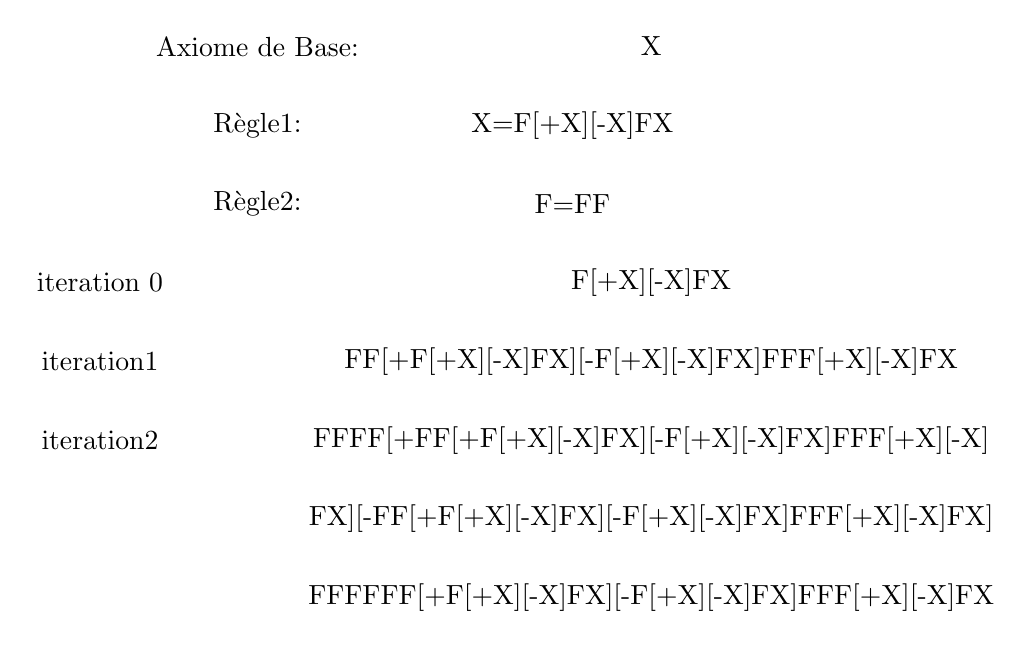
\begin{tikzpicture}
	\node  (base gauche) at (-3,0) {Axiome de Base:};
	\node (base droite) at  (2,0) {X};
	\node (regle1 gauche) at (-3,-1) {Règle1:};
	\node (regle1 droite) at (1,-1) {X={F[+X][-X]FX}};
	\node (regle2 gauche) at (-3,-2) {Règle2:};
	\node (regle2 droite) at (1,-2) {F=FF};
	\node (it0 gauche) at (-5,-3) {iteration 0};
	\node (it0 droite) at (2,-3) {F[+X][-X]FX};
	\node (it1 gauche) at (-5,-4){iteration1};
	\node (it1 droite) at (2,-4){FF[+F[+X][-X]FX][-F[+X][-X]FX]FFF[+X][-X]FX};
	\node (it2 gauche) at (-5,-5) {iteration2};
	\node (it2 droite) at (2,-5) { FFFF[+FF[+F[+X][-X]FX][-F[+X][-X]FX]FFF[+X][-X]};
	\node (it2 droite suite1) at (2,-6) {FX][-FF[+F[+X][-X]FX][-F[+X][-X]FX]FFF[+X][-X]FX]};
	\node (it2 droite suite2) at (2,-7){FFFFFF[+F[+X][-X]FX][-F[+X][-X]FX]FFF[+X][-X]FX};
	\end{tikzpicture}
	\caption{Exemple de génération}\label{figure}

  \end{table}